% =====================================================================
%  MoRE -- TMLR submission (Transactions on Machine Learning Research)
%
%  BUILD:  pdflatex main -> bibtex main -> pdflatex main -> pdflatex main
%          (Overleaf: set the compiler to pdfLaTeX; it runs this for you)
%
%  MODE:   bare \usepackage{tmlr} == ANONYMOUS SUBMISSION.
%          TMLR review is double-blind and submissions MUST be anonymised
%          (jmlr.org/tmlr/author-guide.html). The \author block below is
%          ignored in this mode and replaced by "Anonymous authors / Paper
%          under double-blind review" -- do not remove it, and do not add
%          the [accepted] or [preprint] option until the paper is accepted
%          or you are deliberately posting a non-anonymous preprint.
%
%  PAGE BUDGET: TMLR imposes NO fixed page limit -- "submissions may be any
%          length, but a paper's length should be justified by its content",
%          and unusually long papers risk reviewing delays. The practical
%          norm is ~12 pages of main body. References and appendices sit
%          outside that judgement. This draft is single-column.
%
%  BROADER IMPACT: conditionally required -- only if the work "carries a
%          significant risk of harm". A 5.6M-parameter architecture study on
%          public text does not, so the statement is omitted deliberately
%          rather than forgotten. Revisit if the claim set changes.
%
%  BEFORE SUBMITTING: read VERIFY_BEFORE_SUBMIT.md in this folder. One
%          bibliography entry is knowingly unverified and must be fixed or
%          removed; the build will not warn you about it.
% =====================================================================
\documentclass{article}

\usepackage{tmlr}            % no option == anonymous double-blind submission
% \usepackage[accepted]{tmlr} % camera-ready: reveals authors, adds the header
% \usepackage[preprint]{tmlr} % non-anonymous preprint

% -- tmlr.sty already loads: fancyhdr, natbib, fontenc(T1), lmodern, eso-pic
\usepackage[utf8]{inputenc}
\usepackage{amsmath}         % align/equation; load before \begin{document}
\usepackage{amssymb}
\usepackage{booktabs}        % \toprule \midrule \bottomrule
\usepackage{graphicx}
\usepackage{enumitem}        % \begin{itemize}[leftmargin=...]
\usepackage{microtype}
\usepackage{url}

\graphicspath{{fig/}}

\title{Routing and Recursion Compete: A Parameter-Matched\\
Decomposition of Conditional Computation in Small Language Models}

% Ignored under the anonymous (default) option; fill in for camera-ready.
\author{\name Anonymous Author(s) \email anonymous@example.com \\
        \addr Anonymous Institution}

\begin{document}

\maketitle

\begin{abstract}
Conditional computation is pursued along two axes: sparse mixture-of-experts
(MoE) chooses \emph{which} parameters process a token, and adaptive-depth
weight-tied recursion (MoR) chooses \emph{how much} computation it receives.
The axes are orthogonal, so composing them---routing a token to a specialised
expert and then recursively reusing \emph{that expert's} weights for a learned
number of steps---should inherit both benefits. We test that directly: one
engine, three configurations, parameters matched to 0.069\% ($\approx$5.58M),
bit-identical inputs, five seeds, exact randomisation tests with a
pre-registered correction, on WikiText-103. The composition does not inherit
both. Recursion alone attains the lowest validation loss (3.515 nats/token
against the composition's 3.637 and MoE's 3.948), and adding routing does not
improve routing quality over MoE alone. The sharpest contrast is in adaptive
computation: measured against a \emph{depth-matched} uniform policy, recursion
alone buys 1.47 nats while the composition buys 0.06---a factor of 24---because
the composed model's halting collapses to running to its budget on 97\% of
tokens. We then exclude two explanations. Capacity dilution is arithmetically
ruled out: tokens per parameter are identical across arms by construction, and
once recursion is counted the composed arm receives slightly \emph{more} updates
per parameter than recursion alone. Subspace trapping is falsified three ways:
the recursive arms expand rather than collapse representational dimensionality,
settle rather than oscillate, and update near-orthogonally rather than
rescaling. What the evidence supports is a competition for one per-token
budget---tuning toward adaptive depth destroys expert differentiation, and
preserving differentiation saturates depth. The composition is not uniformly
worse: it is the most robust arm out of domain, beating both components on
held-out text from a different distribution, and it converts compute into
quality roughly three times more efficiently than recursion alone. We report
this as a negative result at this scale, with a falsifiable prediction for the
data scale at which it should reverse.
\end{abstract}

\section{Introduction}
\label{sec:intro}

Conditional computation is usually motivated by the same accounting argument:
most tokens do not need the whole model, so spend less on them. The argument is
made in two places, and the two answer different questions. Sparse
mixture-of-experts (MoE) layers \citep{jacobs1991moe,shazeer2017moe,fedus2022switch}
decide \emph{which} computation module processes a token, dispatching it to one
of several independent sub-networks. Recursive weight-tied architectures with
learned halting \citep{graves2016act,dehghani2019ut,banino2021pondernet} decide
\emph{how much} computation a token receives, reusing one block for a variable
number of steps.

Because the two decisions are made over different objects---which parameters
versus how many applications of them---they are orthogonal in principle, and
composing them is an obvious thing to try. Route a token to a specialised expert,
then reuse \emph{that expert's} weights for as many steps as the token appears to
need. The resulting architecture inherits an efficiency argument from each side.
What it does not inherit is evidence: whether the composition beats either
component at a matched budget has not, to our knowledge, been isolated.

We isolate it. One training engine implements three configurations differing only
in the fields their definitions require: routing without recursion (MoE, six
experts, depth 1), recursion without routing (MoR, one shared block, depth up to
7), and the composition (MoRE, six experts, depth up to 7). All three sit at
$\approx$5.58M parameters, share a bit-identical input representation, and train
on the same fixed split of WikiText-103 \citep{merity2017wikitext} with the same
optimiser budget. Because the comparison is matched rather than merely similar, a
difference between arms cannot be a difference in the harness, the data, or the
parameter count.

\paragraph{What we find.} The composition occupies the compute-efficient point of
the three, and the honest accounting of what it does and does not buy is the
paper.

\begin{itemize}[leftmargin=1.4em,itemsep=1.5pt,topsep=2pt]
\item \textbf{The composition is the most compute-efficient arm.} MoRE improves
  on MoE by $7.9\%$ validation loss ($3.948 \rightarrow 3.637$ nats/token) at
  $2.19\times$ MoE's inference FLOPs, where MoR needs $9.07\times$. It captures
  $72\%$ of MoR's quality gain over MoE for $24\%$ of MoR's inference compute---or
  $15\%$ of its \emph{extra} compute---which is roughly $3\times$ more quality per
  unit of compute than recursion alone, and $6\times$ out of domain.

\item \textbf{And the most robust out of domain.} On held-out text from a
  different distribution \citep{gao2020pile} MoRE is the \emph{best} of the three
  (7.573 nats against MoR's 7.802 and MoE's 8.272), capturing $149\%$ of MoR's
  out-of-domain gain over MoE. The in-domain ordering inverts. This is the one
  respect in which composing the two mechanisms does something neither does alone.

\item \textbf{But recursion alone remains the lowest-loss arm in domain.} MoR
  reaches 3.515 nats/token against MoRE's 3.637---the composition trades
  $0.1216$ nats, significant at our resolution floor, for a $4\times$
  inference-FLOP saving. These are two different axes and we never substitute one
  for the other: at matched parameters MoR wins on quality; per unit of inference
  compute MoRE wins. Adding routing does not improve on recursion alone in domain,
  nor does it improve routing quality over MoE alone.

\item \textbf{Recursion's adaptive depth is real; the composition's barely
  survives.} Against a \emph{depth-matched} uniform policy---forced to the learned
  policy's own mean depth, so total compute is held fixed---MoR's halting buys
  1.47 nats and MoRE's buys 0.06, a factor of 24. MoRE's halting has collapsed to
  running to its budget on 97.3\% of tokens.

\item \textbf{A diagnostic that generalises.} That depth-matched comparison is our
  most transferable contribution. A mean step count and an exit histogram---what
  this literature almost always reports---do \emph{not} establish that depth
  depends on the input; a policy ignoring its input can reproduce both. Scoring
  against a depth-matched uniform policy does, costs one inference pass, and is
  what separates our two arms, which are indistinguishable by mean-and-histogram.

\item \textbf{The two mechanisms compete for one budget.} Depth and
  specialisation are not independent knobs in MoRE the way they are in MoR and
  MoE separately: a calibration sweep that recovers adaptive depth by raising the
  ponder penalty destroys expert differentiation, and the full-corpus arm that
  preserves differentiation saturates depth instead.

\item \textbf{Two explanations are excluded, one by arithmetic.} Capacity
  dilution cannot be the cause: tokens per parameter are identical across arms by
  construction, and once recursion is counted MoRE receives slightly \emph{more}
  updates per parameter than MoR. Subspace trapping is falsified three ways---the
  recursive arms expand rather than collapse representational dimensionality,
  settle rather than oscillate, and update near-orthogonally rather than
  rescaling.
\end{itemize}

We report this as a trade-off measured at this scale rather than as a verdict on
either mechanism in general. The paper's contribution is the decomposition:
because MoE \emph{is} MoRE with the depth budget set to one and all three arms are
parameter-matched from one codebase, each contrast varies one thing. The data
scale at which the surviving account predicts the composition would overtake
recursion alone is stated as a falsifiable claim in \S\ref{sec:limitations}.

\section{Related Work}
\label{sec:related}

\paragraph{Sparse expert routing.}
Conditional mixtures of local experts date to \citet{jacobs1991moe}; the
sparsely-gated form that made them practical at scale is due to
\citet{shazeer2017moe}, with Top-1 dispatch, load-balancing auxiliaries and the
capacity-factor machinery developed in GShard \citep{lepikhin2021gshard}, Switch
Transformer \citep{fedus2022switch} and ST-MoE \citep{zoph2022stmoe}. The standard
justification is more parameters at roughly constant per-token FLOPs. That
argument is unavailable here by construction: we pin all three arms to the same
parameter count, so what remains of the sparsity case is a quality and robustness
case, which \S\ref{sec:results} tests directly.

\paragraph{Adaptive depth and weight-tied recursion.}
Adaptive Computation Time \citep{graves2016act} introduced the learned per-step
halting unit we use; Universal Transformers \citep{dehghani2019ut} applied it to
a weight-tied transformer block, and PonderNet \citep{banino2021pondernet}
reformulated the halting distribution to keep a gradient on the halt head near
saturation. Early-exit variants place the decision at the layer or token level
instead \citep{elbayad2020depthadaptive,schuster2022calm,raposo2024mod}. Weight
tying itself is well established as a parameter-reduction device
\citep{lan2020albert}. What this literature reports is overwhelmingly
\emph{mean} step counts and exit-rate histograms. \S\ref{sec:halting} argues that
neither statistic tests input-dependence, and that the comparison which does---against
the best uniform depth at the same budget---is rarely made.

\paragraph{Composing the two.}
Recent work has begun to combine routing with recursion, most directly by using a
router to assign per-token recursion depth \citep{bae2025mor,raposo2024mod}.
Those systems route \emph{to depths} over shared weights. MoRE differs in that
routing selects among genuinely independent expert FFNs and the recursion then
reuses \emph{that expert's} weights, so the two decisions are made by different
heads over different objects and a token keeps one expert for its whole
trajectory. We are not aware of a matched-budget comparison of such a composition
against each of its components, which is the gap this paper fills. We make no
novelty claim for the combination itself.

\paragraph{Evaluation at small scale.}
Minimal-pair benchmarks \citep{warstadt2020blimp} and likelihood-based world
knowledge probes \citep{ivanova2024ewok} score a \emph{relative} preference within a
matched pair, so they degrade gracefully with model scale rather than collapsing
to chance the way multiple-choice knowledge suites do. At 5.6M parameters they are
the appropriate instrument; \S\ref{sec:results} reports them with the caveat that
our vocabulary is fitted to the training corpus and absolute accuracies are
therefore not comparable to published models.


\section{The MoRE Architecture}
\label{sec:method}

\subsection{Setting and notation}

The task is autoregressive language modelling on packed token sequences. Write
$E$ for the number of experts, $T$ for the maximum recursion depth, $d$ for the
model width, and $\mathbf{h}^{(0)}_s \in \mathbb{R}^{d}$ for the post-embedding
state of position $s$. Unlike a synthetic benchmark, natural language supplies
\emph{no per-token oracle}---neither an expert index nor a complexity label---so
every structural claim below must rest on permutation-invariant statistics or on
comparisons against a controlled alternative. This is why
\S\ref{sec:halting} is built around a forced-depth sweep rather than around
agreement with ground truth.

\subsection{Routing}

Routing happens once per token. A linear router produces
$\mathbf{g} = \mathrm{softmax}(W_r \mathbf{h}^{(0)}_s) \in \Delta^{E-1}$, the
token is assigned to $e^\star = \arg\max_e g_e$, and \emph{only} that expert is
evaluated. The assignment is \emph{persisted}: a token keeps one expert for its
whole recursion trajectory, so the block below reuses one expert's parameters at
every depth and one halt head observes a coherent sequence of states. (An earlier
configuration re-drew both per step; it is retained as a labelled ablation and
discussed in \S\ref{sec:honesty}.)

\begin{equation}
\mathbf{h}^{(t+1)} \;=\; \mathrm{LayerNorm}\!\left(
  \mathbf{h}^{(t)} + g_{e^\star}\cdot \mathrm{FFN}_{e^\star}\!\left(\mathbf{h}^{(t)}\right)
\right), \qquad t = 0,\dots,T-1 .
\label{eq:block}
\end{equation}

The gate probability $g_{e^\star}$ multiplies the expert output, which is what
carries task-loss gradient into the router: the discrete $\arg\max$ is not
differentiated, but the scalar scaling the selected expert's contribution is.
There is one block, so depth is computation through time rather than a stack of
depth-specific layers, and no capacity limit is imposed---every routed token is
evaluated by its expert and none is dropped.

\begin{figure}[t]
    \centering
    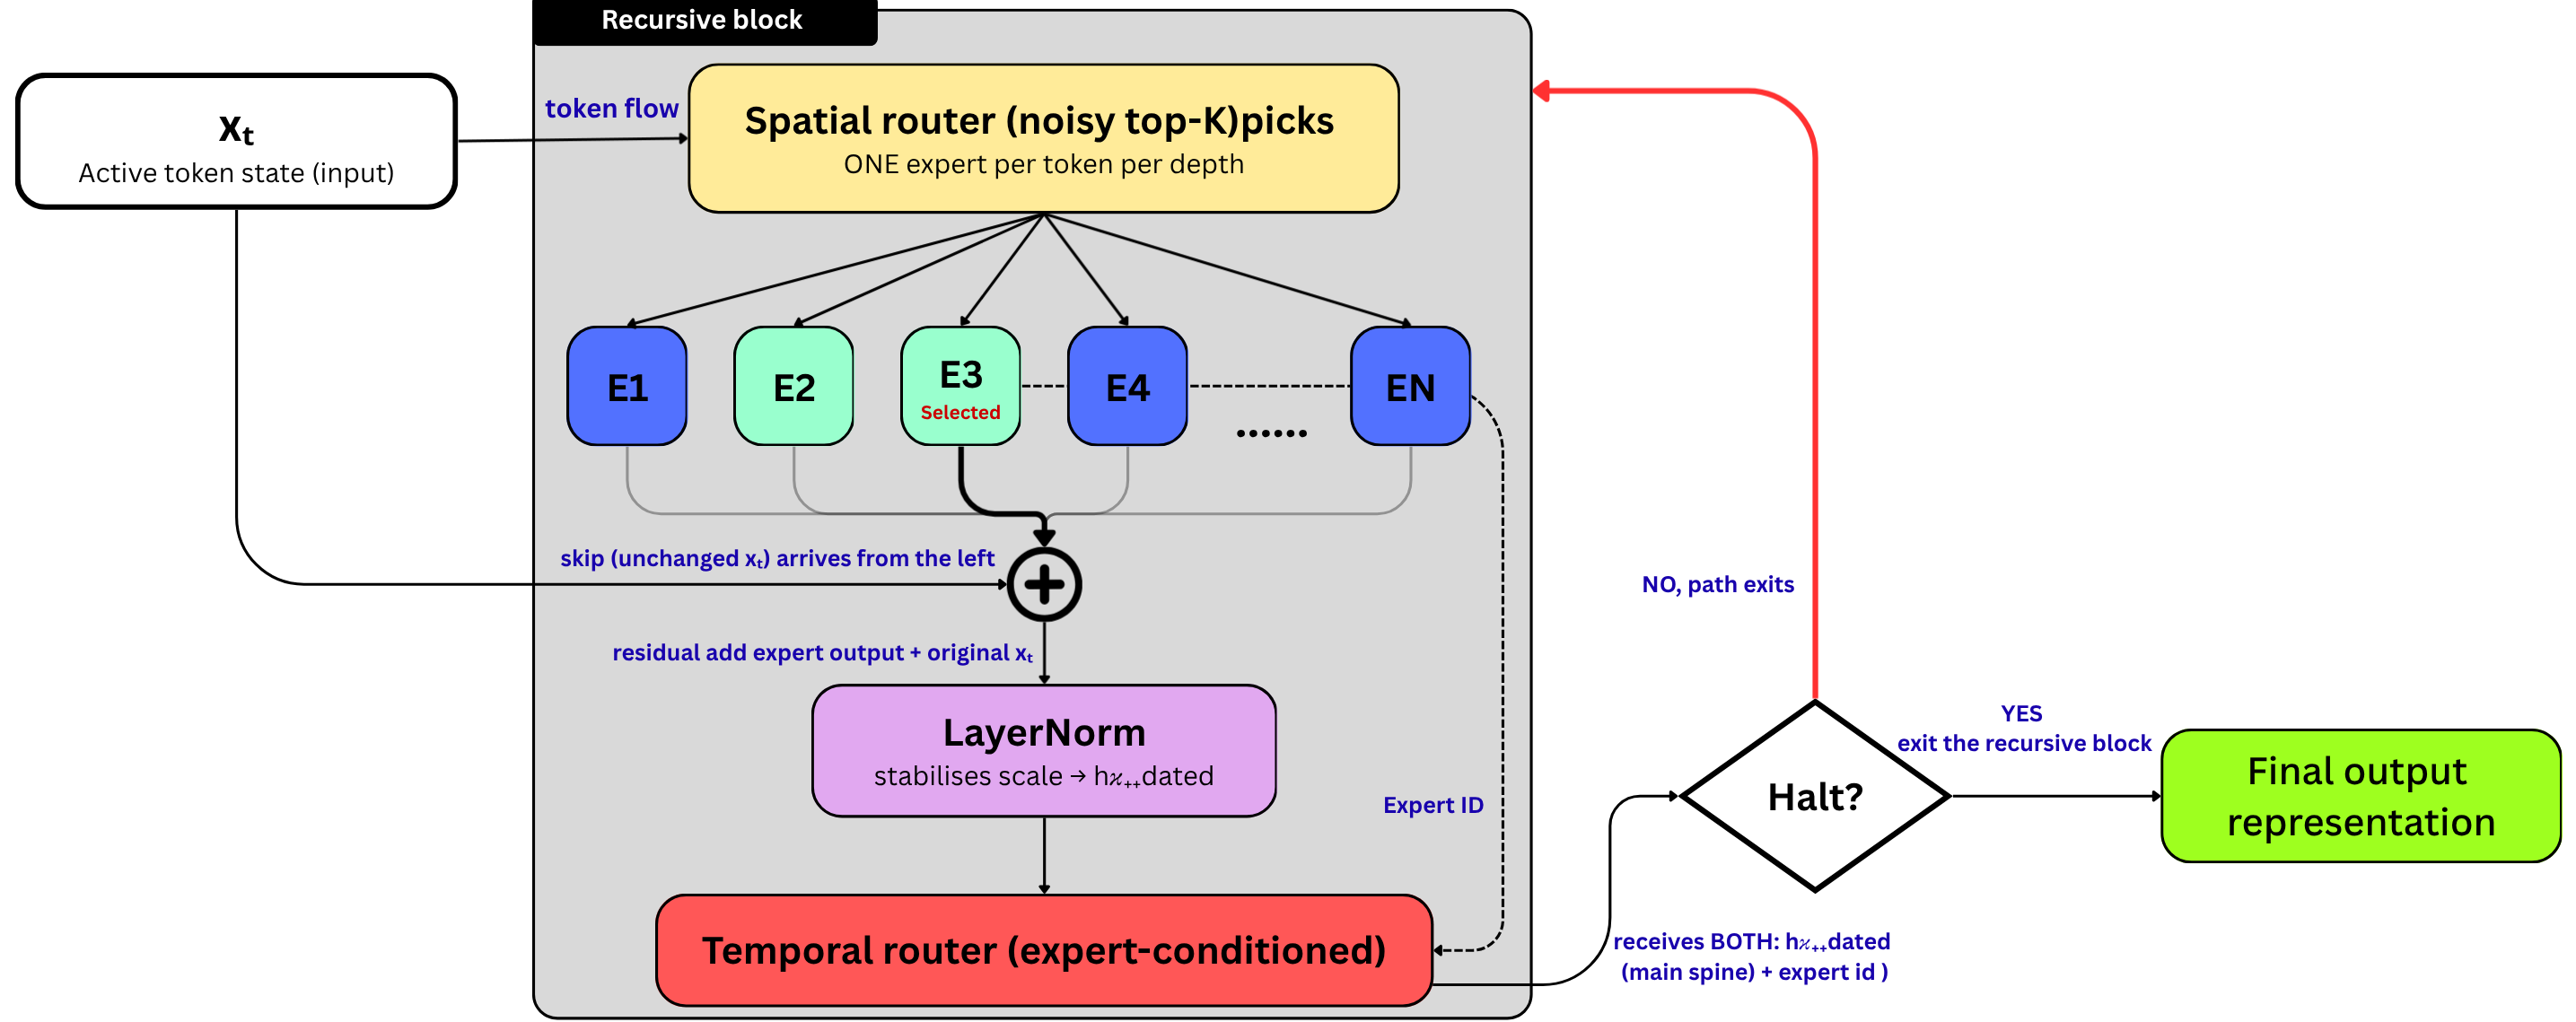
\includegraphics[width=0.86\linewidth,keepaspectratio]{fig_architecture.png}
    \caption{The MoRE block. A token is routed once to one of $E$ independent
    expert FFNs; that expert's weights are then reused for an adaptive number of
    recursion steps under ACT halting. Setting $T=1$ recovers MoE exactly and
    setting $E=1$ recovers MoR; the input representation is bit-identical in all
    three cases.}
    \label{fig:architecture}
\end{figure}

\subsection{Halting and the training objective}
\label{sec:halting-method}

Halting follows ACT \citep{graves2016act} as used in the Universal Transformer,
with one halt head per expert. Per token, at step $t$:

\begin{align}
p_t &= \sigma\!\left(\mathbf{w}_{e^\star}^{\!\top}\mathbf{h}^{(t)}\right),
  & c_t &= \sum_{\tau \le t} p_\tau ,
  \label{eq:halt-p} \\[2pt]
\text{halt when } &\; c_t + p_t > 1 - \epsilon, & \epsilon &= 0.01,
  \label{eq:halt-cond} \\[2pt]
R &= 1 - c_t \ \text{(remainder)}, &
  w_t &= \begin{cases} p_t & \text{running} \\ R & \text{at the halt step}\end{cases}
  \label{eq:halt-w}
\end{align}

and the token's output is the convex combination
$\mathbf{o}_s = \sum_t w_t \mathbf{h}^{(t)}$, whose weights sum to exactly $1$.
That sum-to-one property is the mechanism by which halting is trained: because
$w_t$ scales how much of each step's state reaches the output, changing $p_t$
changes the task loss, so a differentiable path runs from $\mathcal{L}_{\text{task}}$
into the halt parameters. The boolean comparison in
Eq.~\ref{eq:halt-cond} decides dispatch only. Tokens still active at $t=T$ are
forced out; halted states are frozen and not recomputed, so a halted token costs
nothing at deeper steps.

Depth is trained through the expected-depth term
\begin{equation}
\rho \;=\; \mathbb{E}_{\text{tokens}}\big[\,N + R\,\big],
\label{eq:ponder}
\end{equation}
where the step count $N$ is discrete and contributes no gradient while the
remainder $R$ does. Eq.~\ref{eq:ponder} is the ponder cost. It is worth noting
that the gradient reaching the halt heads through $R$ is small compared with the
task gradient: a direct measurement in our implementation puts the halt gradient
at roughly $285\times$ below the task term. This ratio is the quantitative form
of the failure analysed in \S\ref{sec:mechanism}: the ponder term is large enough
to be optimised away but too weak to hold depth down once the task gradient
accumulates, and once the halting sigmoid saturates the gradient through $R$
vanishes \citep{graves2016act}. \citet{banino2021pondernet} is the principled fix
and is future work (\S\ref{sec:limitations}).

The training objective is a weighted sum of terms that we report separately and
never as a single number:
\begin{equation}
\mathcal{L} \;=\;
\underbrace{\mathcal{L}_{\text{task}}}_{1.0} \;+\;
0.001\,\mathcal{L}_{\text{bal}} \;+\;
0.001\,\rho \;+\;
\underbrace{0.0\cdot\mathcal{L}_{\text{fam}}}_{h\,\text{detached}} \;+\;
\underbrace{0.0\cdot\mathcal{L}_{\text{route}}}_{\text{off}} .
\label{eq:loss}
\end{equation}
$\mathcal{L}_{\text{task}}$ is per-token cross-entropy in nats.
$\mathcal{L}_{\text{bal}} = -H(\bar{\mathbf{g}}) + E\sum_e f_e \bar{g}_e$ combines
a router-entropy bonus with the Switch-style auxiliary \citep{fedus2022switch},
where $f_e$ is the dispatched load fraction and $\bar{\mathbf{g}}$ the mean soft
router probability; it is averaged over the depth calls actually made, so its
magnitude does not grow with $T$. Three terms are structurally zero on language
and the reason is not convenience. $\mathcal{L}_{\text{fam}}$ reads
$\mathbf{h}.\mathrm{detach}()$, so its gradient cannot reach the trunk---which
\emph{strengthens} every specialisation claim below relative to a comparable
synthetic study, where a family cross-entropy is typically one of the larger terms
in the objective. $\mathcal{L}_{\text{route}}$ and the halting-supervision term are
zero because natural language supplies no per-token oracle expert and no per-token
oracle depth to supervise against. The canonical router is therefore unsupervised
with respect to the per-token routing decision.

\subsection{One engine, three modes}
\label{sec:engine}

MoE, MoR and MoRE are configurations of one implementation with an explicit
\texttt{architecture} mode, not three codebases. They share one data pipeline, one
optimiser setup and one evaluation path, so a difference between them cannot be a
difference in the harness. Only the fields their definitions require differ:
$E \in \{6,1,6\}$, $T \in \{1,7,7\}$, MoR's FFN multiplier (below), and the two
loss weights for quantities that do not exist in a given arm (no ponder cost at
depth 1, nothing to balance with one expert).

We write \textbf{MoR} for our recursion-only configuration---one shared block with
adaptive halting---which is in the spirit of weight-tied recursive transformers
with learned halting \citep{dehghani2019ut,bae2025mor} but is not a reproduction
of any specific published system; all three arms are configurations of the same
engine.

\paragraph{Matching the budget.} MoR has one FFN where MoRE has six, so matching
the per-FFN multiplier would compare 5.6M parameters against 0.9M and call the
difference architectural. We instead equalise \emph{total} FFN hidden width,
giving MoR's single FFN a multiplier of $24 = 4 \times 6$. The result is
5{,}584{,}908 parameters for MoE and MoRE, identical, and 5{,}581{,}063 for MoR---a
0.069\% deficit that is six per-expert halt heads, the router and FFN biases. That
residual is irreducible at any integer multiplier, and it runs \emph{against} the
headline result: the arm with slightly fewer parameters is the one that wins in
domain.

\section{Experimental Setup}
\label{sec:setup}

\subsection{Data and split}
\label{sec:data}

All arms train on WikiText-103 \citep{merity2017wikitext} with a byte-pair
vocabulary of 8{,}192 tokens and packed sequences of length 256
(\texttt{lang-wikitext-103-bpe8192-len256-800d6154}). We use the corpus's own
author-provided validation split rather than carving one out of the training
material, which is what makes the leakage audit in \S\ref{sec:integrity}
meaningful: no validation or test token was ever available to the trainer.

The baseline floor is a backoff bigram estimated on the same corpus:
\textbf{4.9849 nats/token} (7.19 bits, perplexity 146.2). A model that does not
beat it has learned nothing a two-column count table could not. All three arms
beat it, by margins of $+1.037$, $+1.470$ and $+1.348$ nats for MoE, MoR and MoRE
respectively.

\subsection{Training protocol}
\label{sec:protocol}

Every canonical arm runs at seeds $\{42,43,44,45,46\}$ and is reported as
mean$\,\pm\,$std over five runs. Training is 3 epochs of AdamW (lr $10^{-3}$,
weight decay $10^{-4}$, gradient clipping 1.0, dropout 0.1) with
$d_{\text{model}} = 256$, one block, 4 attention heads, $T = 7$ and batch size 48
on a single laptop GPU. These settings were fixed once, before the comparison, and
not swept per architecture: they are a stable operating point, and no arm was tuned
for itself.

\textbf{Three epochs is a fixed compute budget, not convergence, and we state it
as such.} One epoch is 526{,}320 blocks $\times$ 256 tokens $= 134.7$M tokens
against $\approx$3.4M non-embedding parameters, so the runs sit in an underfitting
regime; the choice of 3 over 2 was made because the halting axis needs more than
two epochs to separate the arms at all, and going to 8 epochs was rejected on cost.
Every arm receives the identical budget, so the comparison is valid even though no
arm is converged. The consequences are stated in \S\ref{sec:limitations}.

\subsection{Metrics}
\label{sec:metrics}

\textbf{Primary metric: validation task loss}, the final-epoch per-token
cross-entropy in nats. We deliberately do not select on best-epoch validation loss:
that is an order statistic whose downward bias scales with each arm's per-epoch
validation noise, which is not matched across architectures. On all 15 cells
\texttt{best} equals \texttt{last}---the evaluation interval is one epoch and the
curves decrease monotonically---so \emph{no model selection occurred} on either
split. Best-epoch values are reported alongside so the selection effect stays
checkable.

Because the router is unsupervised, expert indices carry no semantic identity, so
raw agreement with any externally defined partition measures label permutation as
much as partition quality. We therefore report AMI \citep{vinh2010ami},
Hungarian-matched accuracy and cluster purity, each against a \emph{per-run
permutation control}: the same metric computed against shuffled linguistic labels,
averaged over 10 draws. The controlled quantity is the z-score of the real value
against that null, not the raw value. The externally defined partition is a
part-of-speech hypothesis about a useful expert split---a hypothesis, not a
functional ground truth---so a router can be better for next-token prediction and
still score low against it. We therefore never call this ``routing accuracy''
without that qualifier.

For depth we report mean steps, exit rates, halt mass, and the Spearman correlation
between per-token depth and per-token difficulty. \textbf{The correlation is only
interpretable when depth has variance to correlate}: on an arm whose tokens almost
all exit at the ceiling, the correlation is computed against a near-constant and a
value near zero is uninformative rather than negative evidence. We report the exit
rates next to every correlation for that reason (\S\ref{sec:halting}).

\subsection{Statistics}
\label{sec:stats}

Comparisons use an exact two-sided randomization test on the difference of means,
which enumerates every way of splitting the pooled values into groups of the
original sizes---$\binom{10}{5} = 252$ at five-versus-five---and counts the
fraction whose $|$mean difference$|$ is at least the observed one. It is
exhaustive, hence deterministic: no sampling error, no seed, no normality
assumption, and no threshold to choose. The superseded $k\times$std heuristic is
not used anywhere.

The \textbf{resolution floor} of this design --- the smallest $p$ it can return at
all --- is $2/\binom{n_a+n_b}{n_a}$ for equal arms, which is $2/252 = 0.00794$ at
five-versus-five. The factor of two is there because the two-sided statistic is
invariant under swapping the groups, so extreme regroupings arrive in mirror pairs
and the count at the extreme can never be one.
The argument is worth stating because the floor is a property of the design rather
than of the data. Our statistic is $|\mathrm{mean}(a) - \mathrm{mean}(b)|$. When
the two arms are the same size, the complement of any admissible group-$a$ subset
is itself an admissible group-$a$ subset, and swapping the groups negates the
difference while preserving its absolute value. Every regrouping at the observed
extreme therefore has a partner that is equally extreme, the count can never be
odd at the tail, and the smallest attainable fraction is $2/\binom{n_a+n_b}{n_a}$
rather than $1/\binom{n_a+n_b}{n_a}$. When the arms differ in size the complement
has the wrong size, is not an admissible regrouping, no mirror is forced, and
$1/\binom{n_a+n_b}{n_a}$ becomes attainable.
\textbf{Every headline comparison in this paper sits exactly on that floor}, which
we phrase as ``as extreme as a five-seed design admits''---a weaker statement than
significance, and not to be dressed up as a stronger one. Only more seeds can
strengthen these claims; no larger effect can.

Correction is Holm--Bonferroni over two \emph{pre-registered} families, declared
before the final arm was trained: Family A (predictive quality, $m=4$, metric
validation task loss) and Family B (adaptive depth, $m=2$, metric depth--difficulty
correlation). The split is declared rather than chosen because the two families ask
different questions on different quantities, and pooling them would correct the
depth claim for tests that cannot bear on it. Holm controls the same familywise
error rate as plain Bonferroni and is uniformly more powerful, and here the choice
is load-bearing: plain Bonferroni over the seven comparisons would give
$0.05/7 = 0.00714$, \emph{below} the floor of 0.00794---a design in which no effect
of any size could be declared significant. Holm's easiest threshold at $m=4$ is
$0.0125$, a margin of 0.0046 above the floor.

Two consequences we hold ourselves to. A declared comparison that could not be run
still consumes its slot: dropping a failed arm must never make the survivors easier
to call significant. And a comparison whose floor exceeds its Holm threshold is
\emph{undecidable} and reported \texttt{N/A}, never ``not significant''---that
phrasing would blame the data for a limit of the design.

\subsection{Integrity checks}
\label{sec:integrity}

Three mechanical invariants hold across the matrix, each enforced by an automated
check rather than by inspection. \textbf{(i) Inputs are bit-identical across arms
for the same record}: feature ranges are identical at $E \in \{1,5,6\}$, so a
difference between arms cannot be a difference in representation. \textbf{(ii) The
regression/classification target is absent from the input}, and no oracle routing
label is encoded into a feature slot. \textbf{(iii) The arms are parameter-matched
to 0.069\%} and the seed-blind configuration is identical within each arm, so
comparability cannot rest on a single code revision: the matrix spans four commits,
and it is the frozen specification plus the config-equality check that holds the
arms comparable, not one revision.

One disclosure belongs with the config table. Three loss terms are structurally
zero on language: the family-classification term because its head reads a detached
representation so its gradient cannot reach the trunk, and the routing-supervision
and halting-supervision terms because natural language supplies no per-token oracle
expert and no per-token oracle depth. The first is a genuine advantage over a
comparable synthetic study, where a family cross-entropy is often one of the larger
terms in the objective and every specialisation claim must be caveated for it.

\section{Results}
\label{sec:results}

\subsection{Predictive quality}
\label{sec:quality}

Table~\ref{tab:main} is the headline. Recursion alone is lowest-loss. MoR beats
MoE by $0.4329$ nats and beats MoRE by $0.1216$. Both recursive arms beat MoE
decisively, and the composition lands between them---the premise that routing
would \emph{add} to recursion in domain is not supported.

\begin{table}[t]
\centering
\small
\caption{Canonical results, 5 seeds each, mean$\,\pm\,$std. Primary metric is
final-epoch validation task loss; \emph{best} is the minimum over evaluated
epochs and equals \emph{last} on all 15 cells, so no model selection occurred.
$\Delta$ floor is the margin below the bigram baseline of 4.9849 nats
(positive \emph{beats} it). FLOPs are inference FLOPs/token at each arm's
measured mean depth, from \texttt{results/flops\_language.json}. Pairwise, on the
primary metric: MoRE$-$MoE $-0.3113$ ($d\,{-}15.9$, $p\,0.0079$); MoRE$-$MoR
$+0.1216$ ($d\,{+}4.7$, $p\,0.0079$); MoE$-$MoR $+0.4329$ ($d\,{+}14.7$,
$p\,0.0079$). Exact two-sided randomization test, floor $p_{\min} = 0.00794$;
every headline comparison sits on it.}
\label{tab:main}
\vspace{2pt}
\begin{tabular}{lrrrrrr}
\toprule
& Params & val task loss & PPL & $\Delta$ floor & FLOPs/tok & items/s \\
\midrule
MoE  & 5{,}584{,}908 & 3.9483\,$\pm$\,0.0242 & 51.9 & $+1.0366$ & 5.25\,M & 724 \\
MoR  & 5{,}581{,}063 & \textbf{3.5154\,$\pm$\,0.0340} & \textbf{33.6} & $+1.4695$ & 47.6\,M & 170 \\
MoRE & 5{,}584{,}908 & 3.6370\,$\pm$\,0.0134 & 38.0 & $+1.3480$ & 11.5\,M & 170 \\
\bottomrule
\end{tabular}
\end{table}

Two features of the table deserve to be read together. First, MoE and MoRE are
parameter-\emph{identical} at 5{,}584{,}908 while MoR sits $0.069\%$ lower at
5{,}581{,}063, the residual being the router MoR does not have---and that residual
runs \emph{against} the headline, since the arm with fewer parameters is the one
that wins. Second, MoRE has by far the tightest seed spread (std 0.0134 against
MoR's 0.0340), and we flag that we do not know what to make of it: it is the one
axis on which the composition is unambiguous, and the runs that exist cannot
separate a genuinely stabilising effect from the simpler account that a model whose
halting has collapsed to a constant has less to vary across seeds.

Fig.~\ref{fig:depth-curve} and the forced-depth sweep sharpen this. Both arms scale
with forced depth up to a point, in opposite directions:

\begin{itemize}[leftmargin=1.4em,itemsep=1.5pt,topsep=2pt]
\item \textbf{MoR} improves from 7.36 nats at depth 1 to a minimum of 4.06 at
  depth 4, then \emph{degrades} to 4.99 at depth 7. It has a genuine interior
  optimum.
\item \textbf{MoRE} improves monotonically all the way to depth 7 (3.70), never
  turning over within the budget. It wants more depth than it has.
\end{itemize}

\begin{figure}[t]
\centering
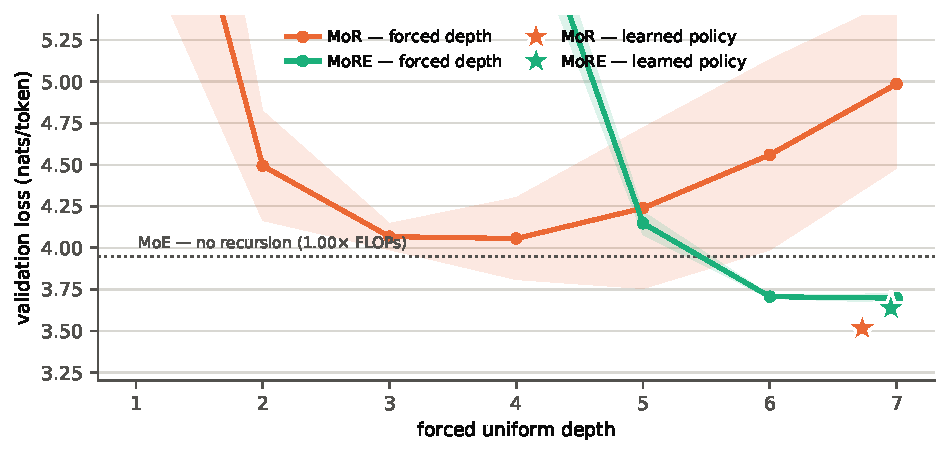
\includegraphics[width=0.92\linewidth]{fig_depth_curve.pdf}
\caption{Validation loss against forced uniform recursion depth, five seeds. Lines
are the forced-depth sweep; stars mark each arm's \emph{learned} policy at its own
measured mean depth. MoR's learned policy sits far below its own best uniform depth
(3.515 vs 4.056); MoRE's sits just below its forced-depth-7 endpoint (3.637 vs
3.697). The dotted line is MoE, which has no recursion. This is the paper's central
contrast: adaptive depth buys MoR a great deal and MoRE very little.}
\label{fig:depth-curve}
\end{figure}

\subsection{Is recursion actually adaptive?}
\label{sec:halting}

The mechanism claim rests on comparing each learned policy against a \emph{uniform}
policy at the same compute, which is the cheapest competitor that ignores its input
and therefore the minimum bar an adaptive-depth claim must clear. Two comparisons
matter, and they give different answers for the two arms.

\textbf{Against the best uniform depth anywhere} (the strongest competitor): MoR's
learned policy at 3.5154 beats its best forced depth (4.0558 at $d{=}4$) by
\textbf{0.540 nats}. MoRE's learned policy at 3.6370 beats its best forced depth
(3.6971 at $d{=}7$) by \textbf{0.060 nats}.

\textbf{Against a depth-matched uniform policy}---forced to exactly the arm's own
measured mean depth of 6.955, so the comparison isolates \emph{where} the compute
goes rather than \emph{how much} there is: MoR's adaptive policy beats forced-$d7$
(4.9863) by \textbf{1.471 nats}; MoRE's beats forced-$d7$ (3.6971) by
\textbf{0.060 nats}.

The depth-matched comparison is the one that licenses a mechanism claim, because
best-depth comparison conflates adaptivity with the average compute spent. On it,
both arms' halting is doing something real and measurable---but MoR's buys 1.47
nats where MoRE's buys 0.06, a factor of roughly 24. The honest summary is not that
MoRE's depth mechanism is inert; it is that adding routing left it almost entirely
without effect.

The exit statistics say why. MoR early-exits $18.8\% \pm 15.1\%$ of validation
tokens with mean depth $6.730$ and a halt remainder of $0.175$;
MoRE force-exits $97.3\% \pm 0.8\%$ at the ceiling with mean depth $6.955$ and
remainder $0.655$. MoRE's halting has collapsed to ``run to budget''.

\textbf{The depth--difficulty correlation is reported next to those rates because
it is only interpretable alongside them.} MoR's per-token depth correlates with
per-token model loss at $\rho = +0.2985 \pm 0.0654$, positive on \textbf{5/5}
seeds. MoRE's is $-0.0230 \pm 0.0115$---but with $97.3\%$ of tokens exiting at the
ceiling and a per-token depth standard deviation of 0.43, that correlation is
computed against a near-constant. We report it as \emph{uninformative}, not as
evidence that MoRE allocates depth badly. This distinction is the paper's most
load-bearing methodological point: a near-zero correlation with a constant is not
a finding about allocation.

MoR's early-exit rate is the seed-unstable quantity ($6.4\%$--$42.2\%$ across
seeds), and its instability is informative. The two seeds that exit most are the
two with the \emph{worst} loss, and the three that exit least are the best. So the
\emph{alignment} of depth with difficulty is robust while the \emph{amount} of
compute skipped is seed-unstable and costs loss---which is why the mean is reported
with its standard deviation rather than as a single depth budget.

\subsection{Where the composition does pay: robustness and efficiency}
\label{sec:ood}

Out of domain the ordering inverts. Table~\ref{tab:evals} evaluates all three arms
on the same checkpoints, and scores each against the inference FLOPs it costs.

\begin{table}[t]
\centering
\small
\caption{Evaluation battery, five seeds. Every cell is
\emph{score (difference vs MoE, inference FLOPs$\times$ vs MoE, difference per
FLOPs-multiplier)}; lower is better for loss rows, higher for accuracy rows.
``diff/$\times$'' is how much score each unit of extra compute bought, so higher is
more efficient. \textbf{These are exploratory}: they sit outside both declared
families, are uncorrected, and carry no significance verdict.}
\label{tab:evals}
\vspace{2pt}
\begin{tabular}{llll}
\toprule
Eval & MoE & MoR & MoRE \\
\midrule
Val loss (nats) & 3.948 (1.00$\times$) & 3.515 ($-0.433$, 9.07$\times$, 0.048) & 3.637 ($-0.311$, 2.19$\times$, \textbf{0.142}) \\
Test loss (nats) & 3.947 (1.00$\times$) & 3.513 ($-0.435$, 9.07$\times$, 0.048) & 3.621 ($-0.326$, 2.19$\times$, \textbf{0.149}) \\
OOD loss (nats) & 8.272 (1.00$\times$) & 7.802 ($-0.470$, 9.07$\times$, 0.052) & \textbf{7.573} ($-0.699$, 2.19$\times$, \textbf{0.319}) \\
BLiMP (acc) & 56.63 (1.00$\times$) & \textbf{58.74} ($+2.11$, 9.07$\times$, 0.233) & 58.36 ($+1.73$, 2.19$\times$, \textbf{0.791}) \\
EWoK (acc) & 49.62 (1.00$\times$)$^{*}$ & 50.33 ($+0.72$, 9.07$\times$, 0.079)$^{*}$ & 49.95 ($+0.33$, 2.19$\times$, 0.152)$^{*}$ \\
\bottomrule
\end{tabular}
\\[3pt]
{\footnotesize $^{*}$EWoK is within noise of the 50\% chance floor for every arm,
so its rankings are not meaningful---a scale limitation, reported for completeness.}
\end{table}

Three things follow.

\textbf{MoRE is the most robust arm out of domain.} On held-out Pile blocks
\citep{gao2020pile} it reaches 7.573 nats against MoR's 7.802 and MoE's 8.272---a
$0.699$-nat advantage over MoE against MoR's $0.470$. The in-domain ordering
inverts: the composition is the \emph{worst} recursive arm in domain and the
\emph{best} out of it. That is a real and reportable property, and it is the one
respect in which composing the two mechanisms does something neither does alone.

\textbf{It gets there far more cheaply.} MoR attains the lowest in-domain loss but
pays $9.07\times$ MoE's inference FLOPs; MoRE pays $2.19\times$. Per unit of extra
compute MoRE buys $0.142$ nats against MoR's $0.048$---roughly $3\times$ the
efficiency in its gain over MoE, and $6\times$ on the OOD row. FLOPs, not
wall-clock, is the compute measure; the throughput column is reported so the
latency cost stays visible, and it shows MoRE no faster than MoR in wall-clock
(170 items/s each) despite doing $4\times$ less arithmetic, because its per-token
expert dispatch is latency-bound.

\textbf{Grammatical competence is real but modest, and routing does not buy it.}
On BLiMP \citep{warstadt2020blimp}, 67{,}000 minimal pairs, both recursive arms beat
MoE (58.74\% and 58.36\% against 56.63\%) and MoR is not distinguishable from MoRE
($p = 0.71$). Every arm is above the 50\% floor, so recursion buys measurable
syntactic sensitivity at this scale; adding routing does not add more of it. The
gains concentrate on long-distance agreement phenomena---anaphor agreement and
determiner--noun agreement---which is where a shared iterative block would be
expected to help. On EWoK \citep{leong2023ewok} all three arms sit at chance, which
is a scale limitation and not a finding.

\subsection{Stratified loss: the advantage concentrates on hard tokens}
\label{sec:stratified}

Fig.~\ref{fig:stratified} groups validation loss by the frequency decile of the
\emph{target} token---difficulty being a property of what must be predicted, not of
the input---and by position within the block.

Both recursive arms improve most where prediction is hardest. The MoRE$-$MoE
advantage grows monotonically from $-0.147$ nats on the rarest-decile tokens to
$-0.374$ on the most frequent; MoR's from $-0.188$ to $-0.527$. Neither
architecture's gain is a uniform shift, which is what a pure capacity effect would
look like.

\begin{figure}[t]
\centering
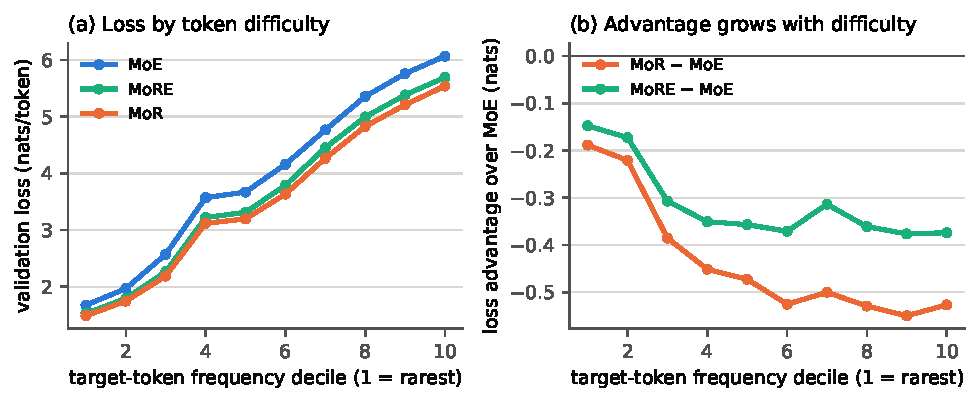
\includegraphics[width=0.98\linewidth]{fig_stratified.pdf}
\caption{(a) Validation loss by target-token frequency decile. (b) Each recursive
arm's advantage over MoE, which widens as tokens get harder. Exploratory,
uncorrected.}
\label{fig:stratified}
\end{figure}

\textbf{A prediction this does not support.} If recursion were doing what the
adaptive-computation premise suggests---spending steps where context is thin---the
recursive arms should gain most at the \emph{start} of a block. They do the
opposite: MoRE's advantage over MoE is $-0.047$ nats in the first 8 positions and
$-0.359$ in the last 128; MoR's goes from $-0.250$ to $-0.465$. Both recursive arms
gain most where context is \emph{longest}. We report this because it disconfirms a
mechanism we would otherwise have asserted, and because it is consistent with the
capacity account in \S\ref{sec:mechanism}: a shared block iterated is accumulating
representation, not compensating for missing context.

\begin{figure}[t]
\centering
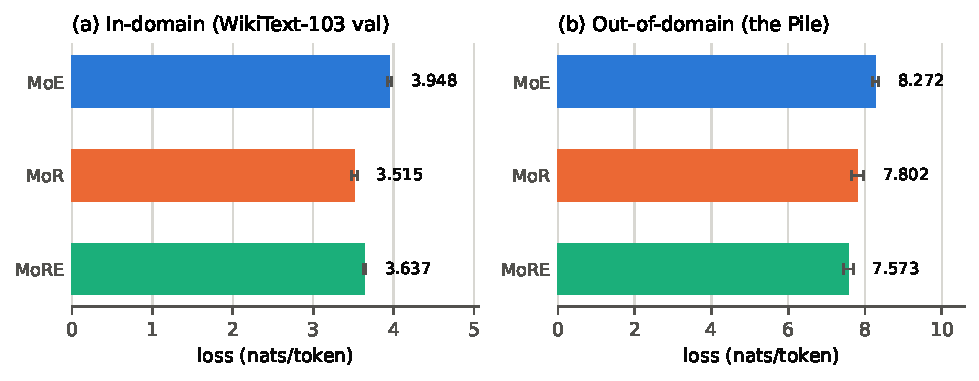
\includegraphics[width=0.98\linewidth]{fig_ood.pdf}
\caption{The ordering inverts out of domain: MoRE is worst in domain (a) and best
on the Pile (b). Same three entities and colours in both panels. Exploratory,
uncorrected.}
\label{fig:ood}
\end{figure}

\section{Why the Composition Fails}
\label{sec:mechanism}

Four accounts, labelled by evidential status: what is measured, and what is
hypothesis consistent with the measurement.

\subsection{Routing divides the data, not the update budget}
\label{sec:dilution}

\textbf{[Ordering MEASURED; arithmetic MEASURED; mechanism HYPOTHESIS.]} The
obvious account of the ordering is capacity dilution: MoR's single block sees
100\% of tokens while MoE and MoRE split the same FFN budget across six experts,
so each expert is trained less. \textbf{That account is arithmetically false
here, and ruling it out is what makes the surviving hypothesis worth stating.}

The budgets are matched by construction, and the matching cancels. Each MoE/MoRE
expert FFN holds $2 \cdot 4 \cdot d^2 = 524{,}288$ weights and MoR's single FFN
holds $2 \cdot 24 \cdot d^2 = 3{,}145{,}728$, exactly six times as many
(\S\ref{sec:engine}). A run sees $404.2$M tokens. So:

\begin{center}
\begin{tabular}{lccc}
\toprule
per FFN parameter & MoE expert & MoR block & MoRE expert \\
\midrule
tokens seen        & 128.5 & 128.5 & 128.5 \\
FFN applications   & 128   & 865   & \textbf{894} \\
\bottomrule
\end{tabular}
\end{center}

Tokens per parameter is \emph{identical} across all three arms---the token split
and the parameter split are both by $E$, so they cancel exactly. And once
recursion is counted, applications per parameter slightly \emph{favours} MoRE
(894) over MoR (865), because MoRE runs marginally deeper. Whatever costs MoRE
0.12 nats against MoR, it is not that its parameters are trained less.

That comparison also explains the easy half of the ordering. MoRE gets
$894/128 \approx 7\times$ the FFN applications per parameter that MoE gets, which
is simply what recursion buys, and MoRE beats MoE by 0.311 nats. The recursive
multiply is real and it is the entire source of MoRE's advantage over MoE.

\textbf{What remains, once update count is excluded, is the \emph{diversity} of
what each parameter block sees.} MoR's block is exposed to the whole token
distribution; each MoE/MoRE expert is exposed only to the router-selected slice
that reaches it, which is both narrower and systematically biased, since the
router selects it. Structure shared across the whole distribution---the bulk of
what a language model must learn at this scale---can be learned once by MoR's
block but has to be re-learned independently inside all six experts. Six partial
copies of shared structure fit in the same parameter budget as one complete copy
only by making each copy worse.

This is a hypothesis, not an isolated effect, and we label it as one: separating
it from the remaining differences needs a width sweep or a controlled
manipulation of routing diversity, and we ran neither. It earns its place because
it is the only account left after the arithmetic above excludes the update-count
version, because it predicts the stratified result---MoRE's advantage over MoE
grows with token difficulty (\S\ref{sec:stratified}), which is where an
incompletely-learned shared structure should hurt most---and because it generates
the falsifiable scale prediction in \S\ref{sec:limitations}: as the corpus grows,
each expert's slice eventually contains enough of the shared structure for the
re-learning penalty to amortise, so the MoR$-$MoRE gap should close with data
scale at fixed parameters.

\subsection{Depth saturation is a data-scale effect, not an architectural limit}
\label{sec:saturation}

\textbf{[MEASURED, four points at fixed hyperparameters.]} MoRE's halting sits at
the ceiling on the full corpus (97.3\% forced-exit, mean depth 6.955 of 7). It is
tempting to read that as the architecture being unable to learn adaptive depth. A
subset sweep falsifies that reading.

\begin{center}
\begin{tabular}{lcc}
\toprule
training data & mean depth & forced-exit rate \\
\midrule
2.5\% of the corpus & 2.43 & $\approx 0$ \\
10\% & 1.92 & $\approx 0$ \\
40\% & 1.97 & $\approx 0$ \\
100\% (canonical) & 6.96 & 0.973 \\
\bottomrule
\end{tabular}
\end{center}

At every reduced-data point the same model, at the same ponder weight, allocates
depth adaptively---exit rates near zero, mean depth between 1.9 and 2.4, inside a
budget of 7. The collapse appears only at full scale. \textbf{So the failure is a
calibration finding, not an architectural one}: the ponder penalty that produces
adaptive depth on a small corpus cannot hold depth down at this one.

We state the limit of that claim precisely, because the sweep is exploratory
(single seed, subset fraction below 1, and it may never be quoted as a canonical
result). The subset axis is \emph{not} cleanly monotone---2.5\% gives 2.43 but 40\%
gives 1.97---so the honest phrasing is that \emph{saturation emerges somewhere
between 40\% and 100\% of the data}, not that depth is monotone in training steps.
The mechanism is consistent: the ponder term is linear in expected depth, while the
task gradient grows as the model fits, so the fixed penalty is outpaced. Once the
halting sigmoid saturates, its gradient vanishes and the linear-penalty ACT scheme
cannot recover on its own \citep{graves2016act}. \citet{banino2021pondernet}
replaces the linear penalty with a KL divergence against a geometric prior, which
keeps a gradient on the halt head near saturation, and is the principled fix; we
did not run it, and it is named as future work rather than as a result.

\subsection{The two mechanisms compete for one budget}
\label{sec:competition}

\textbf{[MEASURED on a calibration grid; the canonical-corpus form is measured on
the balance axis.]} This is the paper's central claim, and it is the one that
explains why the composition does not merely fail to add but subtracts.

Depth and specialisation are not independent knobs in MoRE the way they are in MoR
and MoE separately. On the calibration grid, recovering adaptive depth by raising
the halting weight destroys expert differentiation:

\begin{center}
\begin{tabular}{lccc}
\toprule
halting weight & mean depth & AMI & val loss \\
\midrule
0.001 (frozen) & 2.698 & \textbf{0.2851} & 5.2352 \\
0.107 & 1.476 & \textbf{0.0025} & 5.3346 \\
0.500 & 1.072 & 0.0207 & 5.3306 \\
\bottomrule
\end{tabular}
\end{center}

AMI of 0.0025 is statistically indistinguishable from the shuffled-label control.
The mechanism is direct: fewer recursion steps means fewer expert applications per
token, which means fewer opportunities for experts to differentiate. \textbf{Tune
toward adaptive depth and specialisation collapses; preserve specialisation and
depth saturates.} Both mechanisms draw on the same per-token compute budget, and at
this parameter and data budget neither gets enough. (This grid is on a smaller dev
corpus at one seed; it is a mechanism demonstration and carries that caveat.)

The competition has a second face on the canonical corpus, along a different axis.
The routing balance term is load-bearing and cannot be traded away for depth
either: setting it to zero \emph{collapses} the expert load onto a single expert
(load entropy 0.0001) and drives AMI to zero. A near-uniform per-token router
distribution coexisting with balanced load and above-chance specialisation is
therefore not a pathology to be tuned out---and we note that we initially read it
as one before the sweep refuted us (\S\ref{sec:honesty}).

Specialisation itself is real, and measured against per-run controls rather than
against chance. MoRE's AMI is $0.1803 \pm 0.0246$ against a permutation control of
$0.0249$, a controlled z of $13.43$; Hungarian-matched accuracy is $0.3592 \pm
0.0271$ against a control of $0.2464$. MoE's AMI is $0.1637 \pm 0.0478$ against a
control of $0.0364$ ($z = 6.82$), Hungarian $0.3616$ against $0.2966$. Both
six-expert arms find substantial above-chance structure---and, read together, the
two arms are not distinguishable from each other. Routing quality is approximately
the same with recursion as without it, which is the routing half of the
interference result: recursion does not improve routing, and routing does not
preserve adaptive depth, in the same architecture.

\subsection{A plausible mechanism, refuted}
\label{sec:trapping}

\textbf{[MEASURED; hypothesis falsified.]} The natural explanation for MoRE's
collapse is \emph{subspace trapping}: routing a token once confines its recursion
to a single expert's parameter subspace, and repeated application of one block
within that subspace drives the state toward a fixed point rather than refining it.
It is an appealing account and it is wrong. We tested it three ways.

\begin{center}
\begin{tabular}{lccc}
\toprule
probe & MoE & MoR & MoRE \\
\midrule
final-state participation ratio & $41.5 \pm 1.6$ & $\mathbf{70.3 \pm 5.6}$ & $57.3 \pm 2.8$ \\
between-expert mean cosine & $0.630$ & \textsc{n/a} & $0.916$ \\
\bottomrule
\end{tabular}
\end{center}

\textbf{(i) Trapping predicts lower participation ratio in the composed arm;
it is higher.} If recursion were collapsing the state onto a low-dimensional
subspace, the composed model's final-state PR should fall below MoE's, since MoE
has no recursion at all. It does not: MoRE's PR is $57.3$ against MoE's $41.5$,
and MoR's---with no routing---is higher still at $70.3$. Recursion \emph{expands}
the effective dimensionality, and routing contracts it somewhat without collapsing
it. The ordering refutes the prediction.

\textbf{(ii) Trapping predicts oscillating or fixed-point dynamics; velocity
decays smoothly.} Measuring the L2 norm of consecutive post-norm states across
depth, both recursive arms decay monotonically---MoR from 11.06 at step 2 to 5.71
at step 7, MoRE from 9.09 to 3.49---which is the signature of settling, not of
vibrating around an attractor.

\textbf{(iii) Trapping predicts that successive updates rescale the state;
they are near-orthogonal.} The mean cosine between a step's update and the state
it updates from is negative in both arms ($-0.26$ to $-0.06$), i.e. updates push
into new directions rather than amplifying existing ones. A rescaling collapse
would show positive collinearity approaching $+1$.

The recursion in this architecture is dynamically healthy: it travels, it settles,
and it adds dimensions. The failure is not a broken iterated map. That rules out
the most attractive explanation and leaves the budget competition
(\S\ref{sec:competition}) as the account the data supports---which is a stronger
position than an unexplained null, because we can say which of the obvious
mechanisms it is \emph{not}.


\section{Limitations}
\label{sec:limitations}

\subsection{Scale, stated as a falsifiable prediction}

The study operates at 5.6M parameters, $d_{\text{model}} = 256$, one block, a
vocabulary of 8{,}192, and three epochs of WikiText-103. Sparse-MoE benefits are
known to emerge with scale, so a reviewer can reasonably say the negative result
may be an artefact of operating below the regime where sparsity pays. \textbf{That
objection is correct and cannot be answered with the runs that exist.}

Rather than hedge it, we convert it into the paper's forward claim. The account in
\S\ref{sec:dilution} is that routing divides the \emph{diversity} of data each
parameter block sees, not its update budget---which the arithmetic there shows is
matched exactly. That account predicts a specific crossover: as the corpus grows at
fixed parameters, each expert's router-selected slice comes to contain enough of
the distribution's shared structure that the re-learning penalty amortises, so
\textbf{the MoR$-$MoRE gap should narrow monotonically with training data and the
ordering should eventually invert in favour of the composition}. The out-of-domain
result (\S\ref{sec:ood}) is weak early evidence in this direction, since MoRE is
already the better arm on data it was not trained on.

The measurement that would falsify it: hold parameters, depth budget and optimiser
fixed; sweep training tokens over at least a decade; and report the MoR$-$MoRE gap
as a function of tokens per expert. If the gap is flat or widening, the diversity
account is wrong and the composition's deficit is structural. We did not run that
sweep, and a second model size---the single most valuable follow-up---is likewise
unrun.

\subsection{Budget, not convergence}

Three epochs is a compute budget, and no arm is trained to convergence
(\S\ref{sec:protocol}). This interacts badly with exactly the mechanism the paper
studies: \S\ref{sec:saturation} shows depth allocation is demonstrably
budget-dependent, so the behaviour at 10 epochs is genuinely unknown and might
differ in the direction that matters. Every arm receives the identical budget, so
the comparison is internally valid; the generalisation to trained-to-convergence
models is not established.

Relatedly, one hyperparameter configuration per arm was frozen from a grid run on a
corpus roughly 60$\times$ smaller, and \S\ref{sec:saturation} demonstrates that at
least one weight---the ponder penalty---did not transfer. We did not re-tune per
arm, so the headline ordering could in principle be re-ordered by a per-architecture
search. Given the gaps involved (0.12 nats between the recursive arms), we regard
that as a real risk for the MoR--MoRE comparison and a small one for the comparisons
against MoE.

\subsection{Statistical resolution}

$n = 5$ seeds puts every headline comparison exactly on the design's resolution
floor of $p = 0.00794$ (\S\ref{sec:stats}). ``As extreme as a five-seed design
admits'' is the strongest statement available, and it is weaker than significance.
No larger effect could produce a smaller $p$ here; only more seeds could. Cohen's
$d$ values are reported alongside every gap precisely because a large $d$ on a
small gap is the misreading to avoid---across our own re-exports, $d$ has moved by
a factor of 1.5 while the underlying gap moved by less than 0.005 nats.

\subsection{What was declared and not run}

One comparison in the pre-registered Family A, a depth-matched fixed-depth control,
was declared before results existed and \emph{still consumes its Holm slot}: we do
not delete it to loosen the thresholds on the survivors. The forced-depth sweep in
\S\ref{sec:halting} answers the same question using inference passes over the
canonical checkpoints rather than a trained control arm, so we report it as an
exploratory mechanism result and leave the declared slot consumed and unfilled. A
fixed-depth sweep trained from scratch, a shuffled-depth control, and a
depth--input mutual-information analysis were all declared exploratory and are
unrun.

\subsection{Evaluation caveats}

BLiMP and EWoK are scored with the tokenizer fitted to our training corpus
(8{,}192 BPE merges), so \textbf{absolute accuracies are not comparable to
published models} using 32k--50k vocabularies; only the cross-arm comparison is
valid. EWoK sits within noise of its 50\% chance floor for every arm, which we
report as a scale limitation rather than a result---at 5.6M parameters a world
knowledge probe is below its useful range. All evaluations outside the two declared
families are uncorrected and carry no significance verdict in the abstract or
conclusions.

The perplexities in Table~\ref{tab:main} are intra-study quantities for the same
reason and should not be compared to published WikiText-103 numbers.

\subsection{Disclosures}
\label{sec:honesty}

Several facts about this study would count against it if a reader discovered them
independently, so we state them.

\textbf{An earlier version of the composed arm was not the architecture we define,
and fixing it made our headline worse.} It re-routed at every recursion step,
letting a token traverse up to seven \emph{different} expert FFNs---a heterogeneous
seven-layer network, not one block iterated, and strictly more expressive than the
specification allows. That arm scored 3.5031 and was statistically indistinguishable
from MoR. The architecturally-correct route-once arm reported here scores 3.6370,
\textbf{0.134 nats worse}. The earlier arm's apparent parity with MoR was an
artefact of a specification violation. We retain it unmodified as a labelled
ablation.

\textbf{The pre-registration is partial and the registration file says so itself.}
MoE and MoR were already trained when the test families were declared, so only the
comparisons involving the composed arm are genuinely pre-result. The MoR-versus-MoE
comparison was specified after its data existed, and we do not describe the
registration as complete.

\textbf{We recorded a prediction before the run and it was confirmed.} Before
re-training the route-once arm we predicted in writing that its depth would land
near the cap, specifically so the prediction could not be retrofitted. It came in
at 6.955 of 7.

\textbf{We published a diagnosis that was wrong, and withdrew it.} We initially
read the composed arm's near-maximal per-token router entropy as a balance-loss
pathology and proposed lowering the balance weight. A subsequent sweep refuted
this: at balance weight zero the expert load \emph{collapses} onto one expert and
specialisation goes to zero, so the prescription had the sign backwards. The
underlying error was conflating two quantities---per-token router entropy (0.9999)
with aggregate load entropy (0.9582)---which the tables here keep separate. The
diagnosis is withdrawn and \S\ref{sec:competition} reports what the sweep actually
shows.

\textbf{Provenance is imperfect and we did not retrofit it.} The matrix spans four
code revisions, all with uncommitted working-tree changes at run time;
comparability rests on a frozen specification and a seed-blind configuration-equality
check, not on a single revision. Ten of the fifteen cells predate the fields that
record GPU identity and carry nulls; we did not backfill them, because a provenance
field invented after the fact is worse than an absent one.

\textbf{The matrix spans two GPUs.} Two arms were retrained on one card after the
original checkpoints were lost; the composed arm remains on the original hardware.
We have direct evidence this is benign rather than merely assuming it: both
retrained arms reproduced their published means to $-0.117\sigma$ and $-0.119\sigma$
respectively---agreement to the third decimal across arms that share no
parameters, which is a small \emph{common-mode} offset rather than sampling noise,
and a common-mode shift cancels in the between-arm gaps that carry every verdict
(the MoE$-$MoR gap moved by 0.000185 nats). Per-seed values do \emph{not} reproduce
and we do not claim they do: the seed fixes initialisation, data order and dropout,
but not non-deterministic kernel reduction order. The reproducible quantity is the
arm mean.

\textbf{We report no per-token depth-allocation error.} English supplies no
ground-truth depth per token, so that metric is \texttt{N/A}---not zero. A zero
would read as perfect allocation against a curriculum that does not exist.

\section{Conclusion}
\label{sec:conclusion}

We built the composition of sparse expert routing and adaptive recursion as a
single engine, held parameters and inputs fixed across its three configurations,
and measured what the combination buys at each level of inference compute. At
5.6M parameters on WikiText-103 it buys efficiency and robustness rather than
peak quality. MoRE is the compute-efficient point of the three: $7.9\%$ better
than MoE on validation loss at $2.19\times$ its inference FLOPs, capturing $72\%$
of recursion's quality gain for $24\%$ of recursion's compute, which is roughly
three times more quality per unit of compute. Out of domain it is the best arm
outright, ahead of both components on held-out text from a different
distribution---the one respect in which composing the mechanisms does something
neither does alone.

What it does not buy is in-domain quality. Recursion alone remains lowest-loss by
0.1216 nats, a gap significant at our resolution floor, and adding routing does
not improve routing quality over MoE alone either. We keep the two axes
separate throughout: at matched parameters recursion wins, per unit of inference
compute the composition wins, and neither statement licenses the other. The
composed model's halting still beats a depth-matched fixed policy, so it is not
inert---but it buys 0.06 nats where recursion alone buys 1.47, a factor of 24.

The mechanism is not the obvious one. Routing does not dilute the update budget:
tokens per parameter are identical across arms by construction, and once recursion
is counted the composed arm receives slightly \emph{more} FFN applications per
parameter than recursion alone. Nor is the recursion dynamically broken---we
falsified subspace trapping three ways, finding that the recursive arms expand
rather than collapse representational dimensionality, settle rather than
oscillate, and update near-orthogonally rather than rescaling. What the evidence
supports is a competition for one per-token budget: the two mechanisms cannot both
be tuned up, and the arm that preserves specialisation saturates its depth. If the
surviving diversity account is right, the efficiency-without-peak-quality profile
we measure is what one would expect from an architecture operating below the data
scale at which its routing pays---which is the falsifiable prediction we leave,
with the measurement that would refute it.

We release the engine, the evaluation battery, and the forced-depth control---and
it is the last of these we would most like to see reused. Reporting a mean step
count and an exit histogram, as this literature almost always does, does not
establish that depth depends on the input: a policy that ignores its input can
reproduce both. Scoring a learned policy against a uniform policy forced to the
same mean depth does establish it, costs a single inference pass, and is what
separates our two recursive arms---which are indistinguishable by
mean-and-histogram, and differ by a factor of 24 once the comparison is made. We
would recommend it as a routine check before any model is described as allocating
computation adaptively.


\bibliographystyle{tmlr}
\bibliography{refs}

\end{document}
